\chapter{Аналитический раздел}
\section{Анализ предметной области. Сравнительный анализ существующих решений}
\subsection*{Общая характеристика предметной области}
Цветочный бизнес — это динамично развивающаяся отрасль, включающая продажу свежих цветов, комнатных растений, сопутствующих товаров (упаковка, открытки, удобрения) и дополнительные услуги (доставка). Современные цветочные магазины стремятся автоматизировать процессы учета товаров, управления заказами и взаимодействия с клиентами, что требует эффективных IT-решений.

Ключевые процессы, подлежащие автоматизации:
\begin{itemize}
	\item управление ассортиментом (учет цветов, растений, упаковки);
	\item контроль остатков на складе;
	\item оформление и отслеживание заказов (включая доставку);
	\item управление клиентской базой и маркетинговыми акциями;
	\item аналитика продаж и формирование отчетности;
\end{itemize}

\subsection*{Сравнительный анализ существующих решений}

На рынке представлено несколько типовых решений для автоматизации работы цветочных магазинов:

\begin{enumerate}
\item \textbf{Ручные системы учета} \\
Наиболее простой вариант, включающий использование Excel и бумажных журналов. Основные недостатки: высокая вероятность ошибок при вводе данных и сложности при расширении бизнеса.

\item \textbf{Универсальные CRM-платформы} \\
Такие системы как 1С~\cite{c1} и Битрикс24 предлагают широкий функционал, но их внедрение требует существенных финансовых вложений и часто включает невостребованные возможности.

\item \textbf{Отраслевые программные продукты} \\
Специализированные решения типа FloristWare и FlowerShop Pro созданы специально для флористики, но имеют ограниченную гибкость настройки и высокую стоимость лицензий.
\end{enumerate}


Как показано в таблице~\ref{tab:comparison}, сравнительный анализ существующих решений демонстрирует, что ручные методы учета неэффективны при росте бизнеса из-за высокого риска ошибок и сложности масштабирования. Универсальные CRM-системы (1С, Битрикс24), хотя и предлагают широкий функционал, оказываются избыточными для малого цветочного магазина, требуя значительных затрат на адаптацию. Специализированные решения (FloristWare, FlowerShop Pro), разработанные для флористического бизнеса, часто не покрывают все специфические потребности магазинов и отличаются высокой стоимостью лицензирования.
\begin{table}[h]
	\centering
	\caption{Сравнительный анализ функциональных возможностей систем управления для цветочного бизнеса}
	\label{tab:comparison}
	\begin{tabularx}{\textwidth}{XXXX}
		\toprule
		\textbf{Критерий} & 
		\textbf{Microsoft Excel} & 
		\textbf{1С:Предприятие} & 
		\textbf{FloristWare Pro} \\
		\midrule
		
		\textbf{Автоматизация учета} & 
		Ручной ввод данных, высокая вероятность ошибок & 
		Полная автоматизация всех учетных операций & 
		Специализированная автоматизация для флористики \\
		
		\textbf{Управление складом} & 
		Базовый учет остатков без аналитики & 
		Полноценный складской учет с аналитикой сроков годности & 
		Контроль остатков с напоминаниями о пополнении \\
		
		\textbf{Обработка заказов} & 
		Текстовые записи в ячейках таблицы & 
		Интегрированная CRM-система с историей заказов & 
		Оптимизированный интерфейс для быстрого оформления \\
		
		\textbf{Отчетность} & 
		Ручное составление отчетов по шаблонам & 
		Встроенные отчетные формы с аналитикой & 
		Стандартные отчеты по специфике цветочного бизнеса \\
		
		\textbf{Интеграции} & 
		Ограниченные возможности & 
		Широкие возможности интеграции & 
		Специализированные API для флористики \\
		
		\textbf{Стоимость} & 
		Включена в пакет Office & 
		Лицензия + внедрение) & 
		Подписка \\
		\bottomrule
	\end{tabularx}
\end{table}

\section{Формулировка требований к разрабатываемой базе данных и приложению}
Функциональные требования:
\begin{itemize}
	\item управление товарами (хранение информации о цветах и сопутствующих товарах, учет остатков на складе, обновление количества при поступлении);
	\item управление заказами (регистрация заказов, учет клиентов и истории заказов);
	\item управление поставщиками (ведение списка поставщиков, учет поступлений товаров).
\end{itemize}

\section{Формализация и описание информации, подлежащей хранению в проектируемой базе данных}
Требования к БД:
\begin{itemize}
	\item Сущности:
	\begin{itemize}
		\item Товары (\texttt{id}, название, цена, количество)
		\item Поставщики (\texttt{id}, название, контакты)
		\item Пользователи (\texttt{id}, имя, телефон)
		\item Поставки товаров (\texttt{id}, товары, дата, ответственный)
		\item Заказы (\texttt{id}, клиент\_id, статус, ответственный)
		\item Склады (\texttt{id}, название, адрес)
	\end{itemize}
	
	\item Триггеры:
	\begin{itemize}
		\item автообновление остатков при поставках.
	\end{itemize}
\end{itemize}

\section{Проведенный анализ существующих баз данных на основе формализации данных}
В таблице \ref{tab:db_comparison_BD} представлено сравнение трёх моделей хранения данных: \textbf{SQL (реляционная)}, \textbf{NoSQL (документная)}~\cite{nosql} и \textbf{Ключ-Значение}~\cite{key_value}, проведённое на основе анализа структуры проектируемой базы данных.
\clearpage

\begin{table}[h]
	\centering
	\caption{Сравнение моделей хранения данных}
	\label{tab:db_comparison_BD}
	\begin{tabular}{|p{4cm}|p{3.5cm}|p{3.5cm}|p{3.5cm}|}
		\hline
		\textbf{Критерий} & \textbf{SQL (PostgreSQL, MySQL)} & \textbf{NoSQL (MongoDB)} & \textbf{Ключ-Значение (Redis)} \\
		\hline
		Структура & Жёсткая схема (таблицы) & Гибкая (JSON-документы) & Просто ключ + значение \\
		\hline
		Связи & JOIN, внешние ключи & Вложенные документы & Нет связей \\
		\hline
		Пример для Заказа & Отдельные таблицы (Заказ, Контрагент) & Единый документ с вложенными данными & order:123 → "JSON-данные" \\
		\hline
		Транзакции & Полная поддержка (ACID) & Ограниченная & Нет (или простые операции) \\
		\hline
		Масштабируемость & Вертикальное & Горизонтальное & Горизонтальное \\
		\hline
		Скорость & Оптимизирована для сложных запросов & Быстрые вставки/чтения & Максимальная скорость для простых операций \\
		\hline
		Проблемы & Сложность масштабирования & Дублирование данных & Нет сложных запросов \\
		\hline
	\end{tabular}
\end{table}

Для данной базы данных SQL является оптимальным выбором, так как:
\begin{itemize}
	\item Данные имеют чёткую структуру и связи (например, <<Партия → Номенклатура>>)
	\item Требуются транзакции (например, при списании товаров)
	\item Необходимы сложные запросы с JOIN (анализ продаж, остатков)
\end{itemize}

NoSQL и Ключ-Значение не подходят для основной системы, но могут использоваться как дополнение.

\textbf{Вывод:} реляционная СУБД лучше всего соответствует требованиям данной системы.

\section{ER-диаграмма сущностей проектируемой базы данных в нотации Чена}
На рисунке~\ref{fig:ER} представлена ER-диаграмма сущностей проектируемой базы данных в нотации Чена для разрабатываемого приложения.

\begin{figure}
	\centering
	\includegraphics[width=1\linewidth]{"pictures/ER Chen"}
	\caption{ER-диаграмма сущностей проектируемой базы данных в нотации Чена}
	\label{fig:ER}
\end{figure}


\section{Формализация и описание пользователей проектируемого приложения к базе данных}

\textbf{Пользователи приложения:}
\begin{itemize}
	\item администратор (полный доступ);
	\item продавец (просмотр каталога товаров, работа с заказами);
	\item кладовщик (загрузка информации о новой партии товара, просмотр каталога товаров)
	\end{itemize}

\textbf{Роли БД:}
\begin{itemize}
	\item администратор;
	\item продавец;
	\item кладовщик;
\end{itemize}

\section{Диаграмма вариантов использования}
На рисунке~\ref{fig:UseCase} представлена диаграмма вариантов использования для разрабатываемого приложения.
\begin{figure}
	\centering
	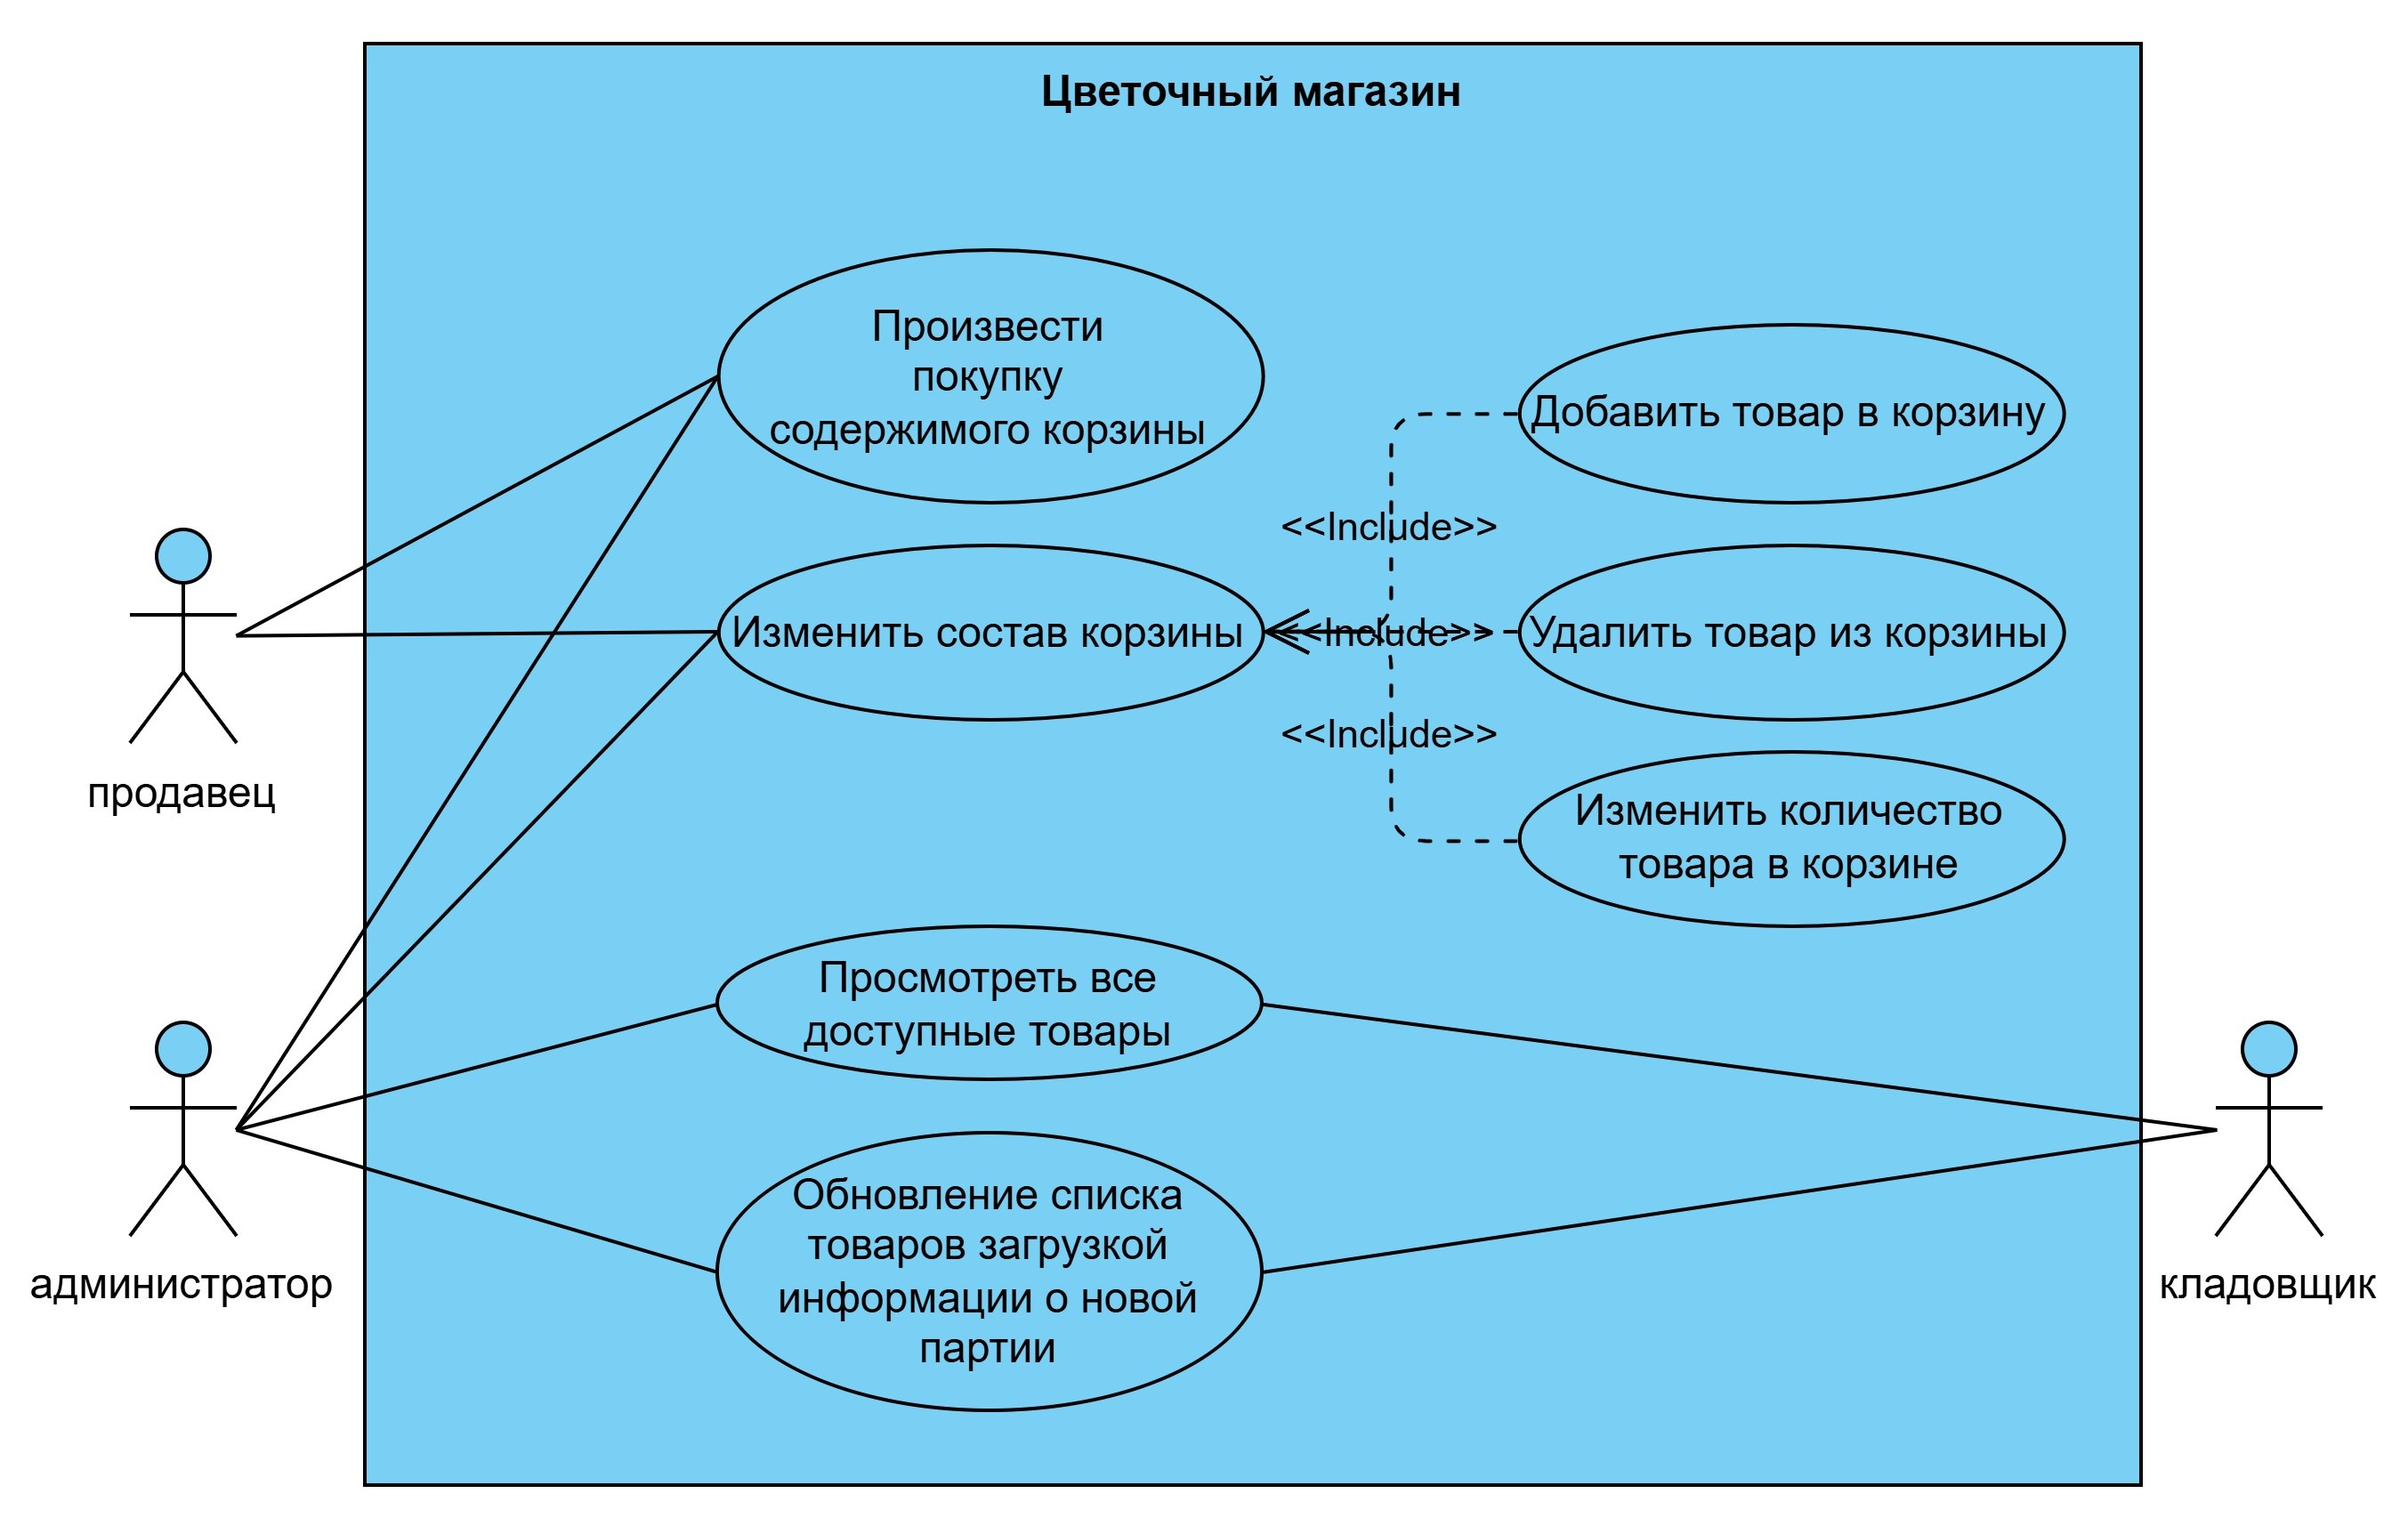
\includegraphics[width=1\linewidth]{pictures/use_case_2}
	\caption{Диаграмма вариантов использования}
	\label{fig:UseCase}
\end{figure}
\section*{Вывод}
Проведённый анализ предметной области и сравнение существующих решений показали необходимость разработки специализированной системы автоматизации для цветочного бизнеса. На основе формализованных требований была спроектирована структура базы данных с чёткими связями между сущностями. Сравнительный анализ моделей хранения данных подтвердил преимущества реляционного подхода, обеспечивающего целостность данных и поддержку транзакций. В качестве СУБД выбрана PostgreSQL, как наиболее подходящая система благодаря её надежности, производительности и богатому функционалу для работы со сложными запросами. Полученные результаты стали основой для дальнейшего проектирования базы данных и разработки приложения.
